\documentclass{article}
\usepackage{amssymb, amsfonts, amsmath}
\usepackage[margin=1in]{geometry}
\usepackage{enumitem}
\usepackage{setspace}
\usepackage{tabu}
\usepackage{graphicx}
\usepackage{setspace}
\usepackage{array}
\usepackage{booktabs}
\usepackage{color}
\usepackage{hyperref}
\hypersetup{urlcolor=blue}
\usepackage{tikz}

\singlespacing
\parindent 0ex
\singlespacing
\parindent 0ex

\def\qed{\hfill$\diamondsuit$}
\newcommand{\vsp}{\vspace{.2in}}
\newcommand{\ed}{\end{document}}
\newcommand{\bear}{\begin{eqnarray*}}
\newcommand{\eear}{\end{eqnarray*}}
\newcommand{\ben}{\begin{eqnarray}}
\newcommand{\een}{\end{eqnarray}}
\newcommand{\bnn}{\begin{enumerate}}
\newcommand{\enn}{\end{enumerate}}
\newcommand{\ds}{\displaystyle}
\newcommand{\im}{\item}
\newcommand{\tabitem}{~~\llap{\textbullet}~~}
\newcolumntype{P}[1]{>{\raggedright\arraybackslash}p{#1}}
\newcommand{\beq}{\begin{equation}}
\newcommand{\eeq}{\end{equation}}
\newcommand{\beqs}{\begin{equation*}}
\newcommand{\eeqs}{\end{equation*}}
\newcommand{\bea}{\begin{align}}
\newcommand{\eea}{\end{align}}
\newcommand{\beas}{\begin{align*}}
\newcommand{\eeas}{\end{align*}}
\newcommand{\bcase}{\begin{cases}}
\newcommand{\ecase}{\end{cases}}
\newcommand{\btab}{\begin{tabular}}
\newcommand{\etab}{\end{tabular}}
\newcommand{\bct}{\begin{center}}
\newcommand{\ect}{\end{center}}
\newcommand{\range}{{\rm Range}}
\newcommand{\var}{{\rm Var}}
\newcommand{\cov}{{\rm Cov}}
\newcommand{\corr}{{\rm Corr}}
\newcommand{\tr}{{\rm tr}}
\newcommand{\questionequal}{\stackrel{?}{=}}
\newcommand{\ncid}{\buildrel d \over \nrightarrow}
\newcommand{\ncip}{\buildrel p \over \nrightarrow}
\newcommand{\cid}{\buildrel d \over \longrightarrow}
\newcommand{\cas}{\buildrel a.s. \over \longrightarrow}
\newcommand{\cw}{\buildrel w \over \longrightarrow}
\newcommand{\cip}{\buildrel p \over \longrightarrow}
%\newcommand{\cil2x}{\buildrel {L_X^2} \over {\longrightarrow}}
%\newcommand{\cil2y}{\buildrel {L_Y^2} \over {\longrightarrow}}
\newcommand{\Ima}{{\rm Im}}
\newcommand{\Sp}{{\rm Span}}
\newcommand{\rank}{{\rm rank}}
\newcommand{\diag}{{\rm diag}}
\newcommand{\proj}{{\rm proj}}
\newcommand{\REF}{{\rm REF}}
\newcommand{\RREF}{{\rm RREF}}
\newcommand{\adj}{{\rm Adj}}
\newcommand{\E}{{\rm E}}
\newcommand{\pbl}{{\pmb l}}
\newcommand{\pbk}{{\pmb k}}
\newcommand{\pby}{{\pmb y}}
\newcommand{\boldalpha}{{\boldsymbol{\alpha}}}
\newcommand{\boldbeta}{{\boldsymbol{\beta}}}
\newcommand{\boldrho}{{\boldsymbol{\rho}}}
\newcommand{\bgamma}{{\boldsymbol{\gamma}}}
\newcommand{\boldepsilon}{{\boldsymbol{\varepsilon}}}
\newcommand{\bbetahat}{{\hat{\boldsymbol{\beta}}}}
\newcommand{\bepsilonhat}{{\hat{\boldsymbol{\varepsilon}}}}
\newcommand{\bnuhat}{{\hat{\boldsymbol{\nu}}}}
\newcommand{\CK}{{\cal K}}
\newcommand{\CA}{{\cal A}}
\newcommand{\CB}{{\cal B}}
\newcommand{\CC}{{\cal C}}
\newcommand{\CI}{{\cal I}}
\newcommand{\CP}{{\cal P}}
\newcommand{\CF}{{\cal F}}
\newcommand{\CG}{{\cal G}}
\newcommand{\CU}{{\cal U}}
\newcommand{\CM}{{\cal M}}
\newcommand{\CN}{{\cal N}}
\newcommand{\CR}{{\cal R}}
\newcommand{\CH}{{\cal H}}
\newcommand{\CE}{{\cal E}}
\newcommand{\CL}{{\cal L}}
\newcommand{\CO}{{\cal O}}
\newcommand{\CT}{{\cal T}}
\newcommand{\CW}{{\cal W}}
\newcommand{\CY}{{\cal Y}}
\newcommand{\CZ}{{\cal Z}}
\newcommand{\BBC}{{\mathbb C}}
\newcommand{\BBN}{{\mathbb N}}
\newcommand{\BBZ}{{\mathbb Z}}
\newcommand{\BBR}{{\mathbb R}}
\newcommand{\BA}{{\mathbf{A}}}
\newcommand{\BB}{{\mathbf{B}}}
\newcommand{\BC}{{\mathbf{C}}}
\newcommand{\BD}{{\mathbf{D}}}
\newcommand{\BE}{{\mathbf{E}}}
\newcommand{\BF}{{\mathbf{F}}}
\newcommand{\BG}{{\mathbf{G}}}
\newcommand{\BH}{{\mathbf{H}}}
\newcommand{\BI}{{\mathbf{I}}}
\newcommand{\BJ}{{\mathbf{J}}}
\newcommand{\BK}{{\mathbf{K}}}
\newcommand{\BL}{{\mathbf{L}}}
\newcommand{\BM}{{\mathbf{M}}}
\newcommand{\BN}{{\mathbf{N}}}
\newcommand{\BO}{{\mathbf{O}}}
\newcommand{\BP}{{\mathbf{P}}}
\newcommand{\BQ}{{\mathbf{Q}}}
\newcommand{\BR}{{\mathbf{R}}}
\newcommand{\BS}{{\mathbf{S}}}
\newcommand{\BT}{{\mathbf{T}}}
\newcommand{\BU}{{\mathbf{U}}}
\newcommand{\BV}{{\mathbf{V}}}
\newcommand{\BW}{{\mathbf{W}}}
\newcommand{\BX}{{\mathbf{X}}}
\newcommand{\BY}{{\mathbf Y}}
\newcommand{\BZ}{{\mathbf{Z}}}
\newcommand{\CS}{{\cal S}}
\newcommand{\FC}{\field{C}}
\newcommand{\la}{{\langle}}
\newcommand{\ra}{{\rangle}}
\newcommand{\bu}{\mathbf{u}}
\newcommand{\ba}{\mathbf{a}}
\newcommand{\bb}{\mathbf{b}}
\newcommand{\bc}{\mathbf{c}}
\newcommand{\bd}{\mathbf{d}}
\newcommand{\be}{\mathbf{e}}
\newcommand{\bbf}{\mathbf{f}}
\newcommand{\bg}{\mathbf{g}}
\newcommand{\bh}{\mathbf{h}}
\newcommand{\bi}{\mathbf{i}}
\newcommand{\bj}{\mathbf{j}}
\newcommand{\bk}{\mathbf{k}}
\newcommand{\bbm}{\mathbf{m}}
\newcommand{\bn}{\mathbf{n}}
\newcommand{\bo}{\mathbf{o}}
\newcommand{\bp}{\mathbf{p}}
\newcommand{\bq}{\mathbf{q}}
\newcommand{\br}{\mathbf{r}}
\newcommand{\bs}{\mathbf{s}}
\newcommand{\bt}{\mathbf{t}}
\newcommand{\bfu}{\mathbf{u}}
\newcommand{\bv}{\mathbf{v}}
\newcommand{\bw}{\mathbf{w}}
\newcommand{\bx}{\mathbf{x}}
\newcommand{\by}{\mathbf{y}}
\newcommand{\bz}{\mathbf{z}}
\newcommand{\bmu}{\mathbold{\mu}}
\newcommand{\BSigma}{\mathbold{\Sigma}}
\newcommand{\boldK}{\mathbf{K}}
\newcommand{\bKX}{\mathbf{K_X}}
\newcommand{\bKY}{\mathbf{K_Y}}
\newcommand{\bKXY}{\mathbf{K_{XY}}}
\newcommand{\bKYX}{\mathbf{K_{YX}}}
\newcommand{\boldX}{\mathbf{X}}
\newcommand{\boldL}{\mathbf{L}}
\newcommand{\boldP}{\mathbf{P}}
\newcommand{\boldY}{\mathbf{Y}}
\newcommand{\boldT}{\mathbf{T}}
\newcommand{\bolda}{\mathbf{a}}
\newcommand{\boldb}{\mathbf{b}}
\newcommand{\bolde}{\mathbf{e}}
\newcommand{\boldu}{\mathbf{u}}
\newcommand{\boldv}{\mathbf{v}}
\newcommand{\boldf}{\mathbf{f}}
\newcommand{\boldD}{\mathbf{D}}
\newcommand{\boldx}{\mathbf{x}}
\newcommand{\boldy}{\mathbf{y}}
\newcommand{\boldg}{\mathbf{g}}
\newcommand{\boldt}{\mathbf{t}}
\newcommand{\boldV}{\mathbf{V}}
\newcommand{\boldA}{\mathbf{A}}
\newcommand{\boldB}{\mathbf{B}}
\newcommand{\boldW}{\mathbf{W}}
\newcommand{\bbeta}{{\boldmath \beta}}
\newcommand{\balpha}{{\boldmath \alpha}}
\newcommand{\boldeta}{{\boldmath \eta}}
\newcommand{\boldnu}{{\boldmath \nu}}
\newcommand{\tcr}{\textcolor{red}}
\newcommand{\tcb}{\textcolor{blue}}
\def\II{I\negthinspace I}
\def\III{I\negthinspace I\negthinspace I}
\newcommand{\bepsilon}{{\mathbf \varepsilon}}
\newcommand{\ep}{\vskip-.3cm\noindent\begin{flushright}
${{\hfill\llap{$\sqcup\!\!\!\!\sqcap$}}}$
\end{flushright}}

\newcommand{\pl}{\parallel}
\newcommand{\fin}{\ \ \rule{2mm}{2mm}}
\newcommand{\limi}{{\ds \lim_{i\rightarrow\infty}}}
\newcommand{\limn}{{\ds \lim_{n\rightarrow\infty}}}
\newcommand{\es}{\hspace*{0mm}}
\def\rit{\hbox{\it I\hskip -2pt R}}
\def\nit{\hbox{\it I\hskip -2pt N}}
\def\cit{\hbox{\it l\hskip -5.5pt C}}
\def\zit{\hbox{\it Z\hskip -4pt Z}}
\def\qit{\hbox{\it l\hskip -5.5pt Q}}

\usepackage{Sweave}
\begin{document}
\Sconcordance{concordance:EDA_Midterm_Exam.tex:EDA_Midterm_Exam.Rnw:%
1 212 1 1 0 224 1 1 2 1 0 4 1 4 0 1 2 33 1 1 2 1 0 1 1 1 3 2 0 1 1 1 2 %
1 0 1 2 1 0 1 2 1 0 1 3 2 0 1 1 1 2 1 0 1 3 2 0 1 3 2 0 1 1 1 3 1 0 1 2 %
1 0 1 1 1 2 7 0 1 5 18 1}

\begin{flushright}
\begin{tabular}{p{3in} p{3in} r }
\textbf{STAT-S 470/670 EDA} & \textbf{Midterm} & \textbf{10/23/15}\\
\hline
\end{tabular}\\
\end{flushright}

\textbf{Ganesh Nagarajan, gnagaraj at indiana.edu}\\ \vskip 0.5 em

\begin{enumerate}
\item During the winter of 1893--1894, the chemist Lord Rayleigh
was studying the density of nitrogen from various sources.
Here are his measurements on the density of N$_2$.


\begin{verbatim}
         1       2       3       4       5       6       7       8
   2.30143 2.29816 2.30182 2.29890 2.31017 2.30986 2.31010 2.31001
         9      10      11      12      13      14      15
   2.29889 2.29940 2.29849 2.29889 2.31024 2.31030 2.31028
\end{verbatim}

For your convenience, below are the data after subtracting 2.30
and multiplying by $10^5$:

\begin{verbatim}
      1    2    3    4    5    6    7    8    9   10   11   12   13   14   15
day   1    7    8   10   14   16   21   24   28   30   42   46   60   63   65
wt2 143 -184  182 -110 1017  986 1010 1001 -111  -60 -151 -111 1024 1031 1028
\end{verbatim}

\begin{enumerate}
\item (10 points) Calculate the five number summary for these data. % Specify their depths.
(You may use wt2 data.) \vskip 1.7in


\item Using your five-number summary, construct the stem and leaf display and then draw the
boxplot.  Are there any outliers?  (It will take less space if you draw the
box horizontally)

\end{enumerate}


\newpage
\item If you had a sample $n=5000$ from a Gaussian distribution, approximately how many ``outside values'' would you expect in a boxplot? \vskip 1in

\item Indicate which of the following would or would not need a re-expression. For those situations that do indicate re-expression, \textbf{describe} the tool you would use to identify it. [If the tool is a plot, state the quantities on the x- (horizontal) and y- (vertical) axes.]


\begin{enumerate}
\item
\begin{verbatim}
 The decimal point is 1 digit(s) to the left of the |

  22 | 6
  24 |
  26 |
  28 | 46
  30 | 39
  32 | 2301
  34 | 66034
  36 | 388238
  38 | 13333455578913455689
  40 | 14566822455699
  42 | 01246699911233557888
  44 | 001234662225668999
  46 | 4556800
  48 | 8

\end{verbatim}


\item 5 boxplots of 5 samples show F-spreads of 13, 1, 10, 8, 4


\newpage
\item Normal QQ plot looks like this:\\
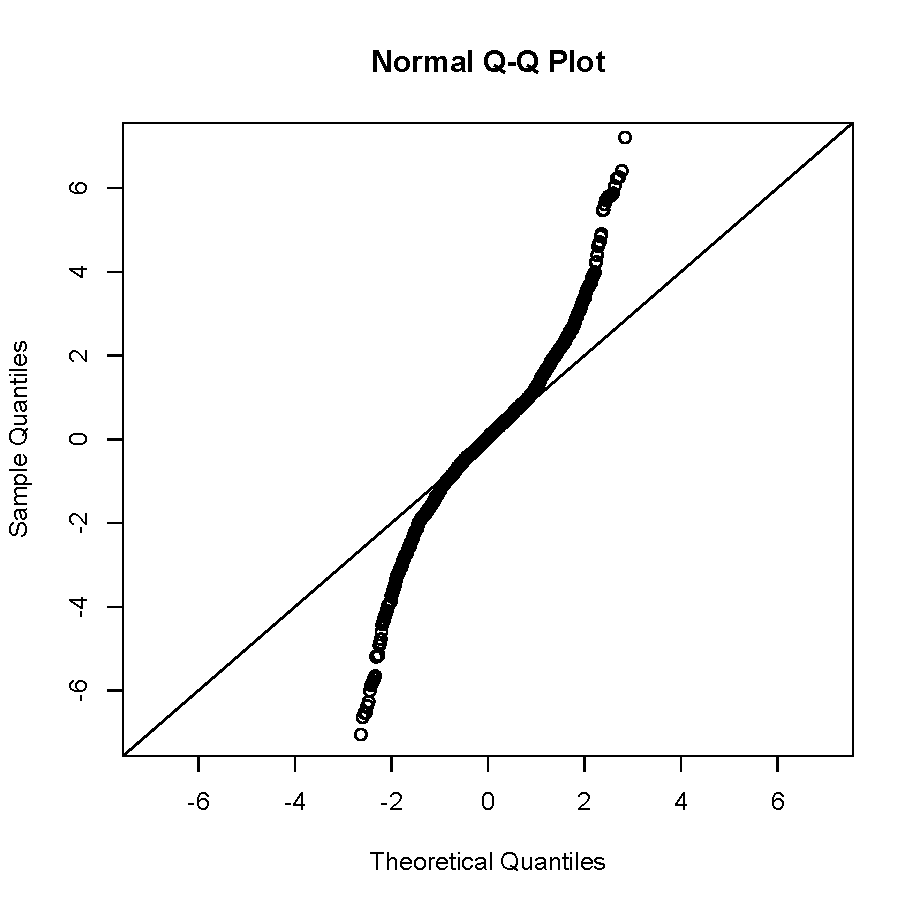
\includegraphics[scale=0.5]{qqplot1}

\item Normal QQ plot looks like this:\\
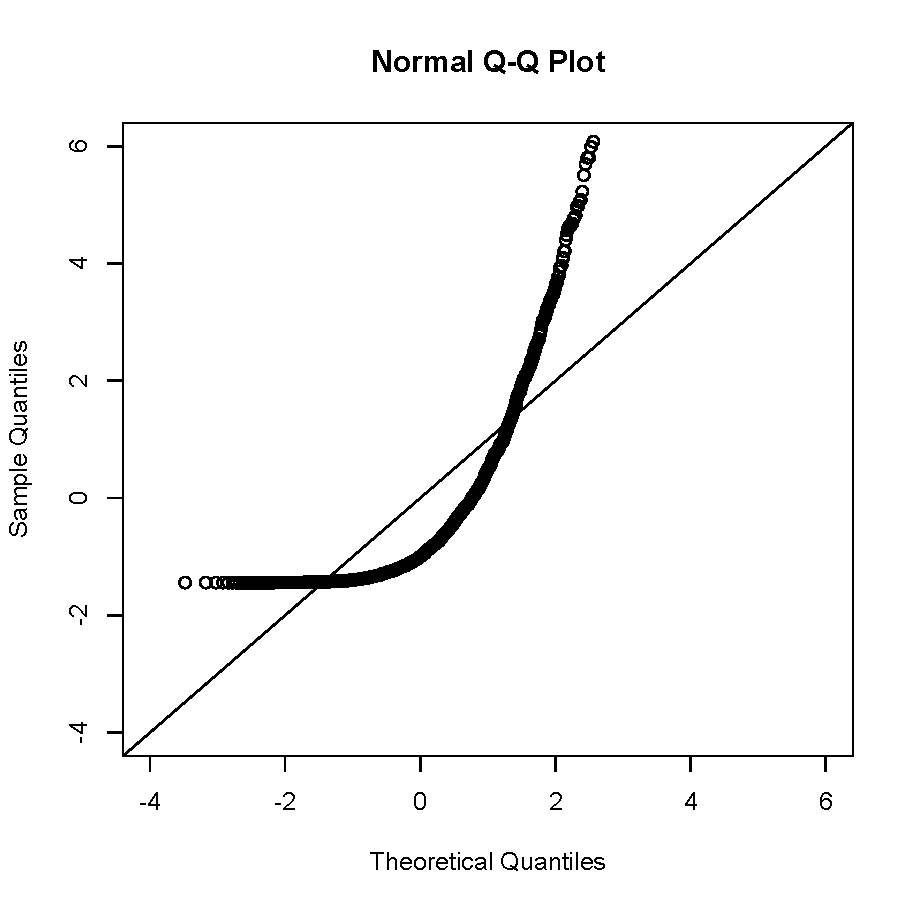
\includegraphics[scale=0.5]{qqplot2}
\end{enumerate}

\item What is a linear smoother? Give names for two linear smoothers. What are the problems with linear smoothers?  State at least 1 advantage and 1 disadvantage of nonlinear smoothers over linear smoothers.


\newpage


\item Below are data from an experiment to measure storage and transport of calcium in cells across cell membranes. time refers to the number of minutes that the cells were suspended in a solution; cal denotes the amount of calcium that was absorbed by the cells during that time. For your convenience, data are ordered by the time variable.

\begin{verbatim}
          1      2      3      4      5      6      7     8      9
time  0.450   0.45  0.450  1.300  1.300  1.300  2.400 2.400  2.400
cal   0.342   0.00  0.825  1.780  0.954  0.641  1.751 1.275  1.173
         10     11     12     13     14     15     16    17     18
time  4.000   4.00  4.000  6.100  6.100  6.100   8.05 8.050  8.050
cal   3.123   2.61  2.574  3.179  3.008  2.671   3.06 3.943  3.437
         19     20     21     22     23     24     25    26     27
time 11.150 11.150 11.150 13.150 13.150 13.150 15.000 15.00 15.000
cal   4.807  3.356  2.783  5.138  4.703  4.257  3.604  4.15  3.425
\end{verbatim}

A plot of the data appears in panel (a) in the figure below.

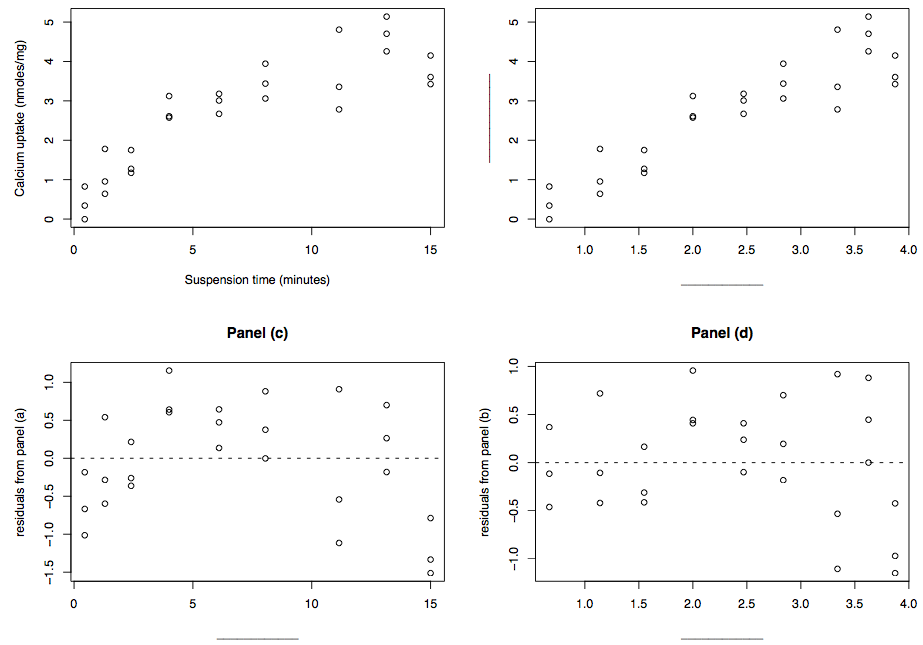
\includegraphics[scale=0.5]{lineplot}

\begin{enumerate}
\item (10 points) Calculate the initial slope of the RR line. For the initial intercept, you may use one of the formulas you learned in class (choose wisely and state which one you use).
\begin{verbatim}


     Intercept = ________    Slope = ________

\end{verbatim}

\item If the plot does not look straight, what �rule� would you use or what do you do to straighten the plot? \vskip 0.8in
\item Panel (b) plots the data again, with one or both of the axes transformed. Can you determine which transformation(s) were applied? If you cannot name the exact one(s), can you use part (b) above to assess the direction of the transformation(s)?\vskip 1in
\item Graphically place an initial RR line on Fig (b), and estimate its slope and intercept.
\begin{verbatim}


     Intercept = ________    Slope = ________

\end{verbatim}

\item Panels (c) \& (d) show the residual plots from the initial RR lines in each case. Briefly comment on these two residual plots. \vskip 1.5in


\item Suppose the slope \& intercept of an RR line were calculated for the data from residual plot (d).
\begin{verbatim}
     Intercept = 0.256   Slope = -0.124
\end{verbatim}


Using the above results, what are the final slope and intercept from the two iterations?
\begin{verbatim}


     Intercept = ________    Slope = ________

\end{verbatim}
\end{enumerate}



\newpage
\item A client to our Statistical Consulting Class last spring counted
numbers of visits by flying insects to her plants having
red, white, or pink flowers (``treatments'') which had been
placed in five different areas.
Below are the average counts (\#visits) collected at 5 different areas
on the three types of plants:

\begin{verbatim}
           Area
      | A1   A2   A3   A4   A5
   ----------------------------
   T1 |  5    6    3   11   10
   T2 | 14   10    6   12   21
   T3 | 16   24   15   26   32
\end{verbatim}

\begin{enumerate}
\item (10 points) Conduct median polish on this table.
In the table below, provide the row, column, and common effects,
as well as the residuals.  What do the effects suggest?\\\vskip 0.2em
Median Polish Fit\\
\begin{tabular}{c|ccccc|c}
& A1 & A2 & A3 & A4 & A5 & Row \\ \hline
T1 &&&&&\\
T2 &&&&&\\
T3 &&&&&\\ \hline
Col &&&&&\\
\end{tabular}

\item How ``good'' is the median polish fit?  Calculate a
statistic that gives a rough indication of the ``quality'' of the fit.
(Hint: The median of the raw data is 12.) \vskip 1in

\item What is the diagnostic plot?  (State how it is constructed.)
What does it tell you? \vskip 1.5in


\item Construct the ``forget-it" plot (on graph paper); show the y-axis.
Show on the plot how to read off the fitted value
for Area A4 using Treatment T3. %(easy to do)

\end{enumerate}



\item  The following data come from a regression example in the text
non-parametric regression and spline smoothing (Eubank, 1988).  

\begin{tabular}{|cc|cc|cc|cc|}
\hline
t & y & t & y & t & y & t & y \\ 
\hline .010 & -.0937 & .030 & .0247 & .050 & .1856 & .070 & .1620 \\
.090 & -.0316 & .110 & .1442 & .130 & .0993 & .150 & .3823 \\
.170 & -.0624 & .190 & .3262 & .210 & .1271 & .230 & -.4158 \\
.250 & .0975 & .270 & -.0836 & .290 & .7410 & .310 & .3749 \\
.330 & .4446 & .350 & .5432 & .370 & .6946 & .390 & .5869 \\
.410 & .9384 & .430 & .7647 & .450 & .9478 & .470 & .9134 \\
.490 & 1.2437 & .510 & .9070 & .530 & 1.2289 & .550 & .9638 \\
.570 & .8834 & .590 & .6982 & .610 & .5729 & .630 & .7160 \\
.650 & 1.0083 & .670 & .6681 & .690 & .5964 & .710 & .4759 \\
.730 & .6217 & .750 & .6221 & .770 & .6244 & .790 & .5918 \\
.810 & .7047 & .830 & .5234 & .850 & .9022 & .870 & .9930 \\
.890 & .8045 & .910 & .7858 & .930 & 1.1939 & .950 & .9272 \\
.970 & .8832 & .990 & .9751 & & & & \\
\hline
\end{tabular}

This data was generated using the model 
$$ y(t_i) = \mu( t) + \varepsilon_i $$
where $ \varepsilon_i \sim N( 0, \sigma^2)$ was generated using rnorm()
for some $\sigma$ and the true mean function was given by

$$  \mu(t) = t + 0.5 \exp(-50(t- 0.5)^2 ) $$

Note that in real life you would not know the true mean function fut have to guess at it. In R you can load in the data by executing the following commands.

\begin{Schunk}
\begin{Sinput}
> x = seq(0.01,0.99,by=0.02)
> y=c(-0.0937,0.0247,0.1856,0.1620,-0.0316, 0.1442,0.0993,0.3823,-0.0624,0.3262,0.1271,-0.4158,0.0975,-0.0836,0.7410,0.3749,0.4446,0.5432,0.6946,0.5869,0.9384,0.7647,0.9478,0.9134,1.2437,0.9070,1.2289,0.9638,0.8834,0.6982,0.5729,0.7160,1.0083,0.6681,0.5964,0.4759,0.6217,0.6221,0.6244,0.5918,0.7047,0.5234,0.9022,0.9930,0.8045,0.7858,1.1939,0.9272,0.8832,0.9751)
> mu = function(t){t + 0.5 *exp(-50*(t-0.5)^2)}
> curve(mu(x),0,1)
> points(x,y)
\end{Sinput}
\end{Schunk}
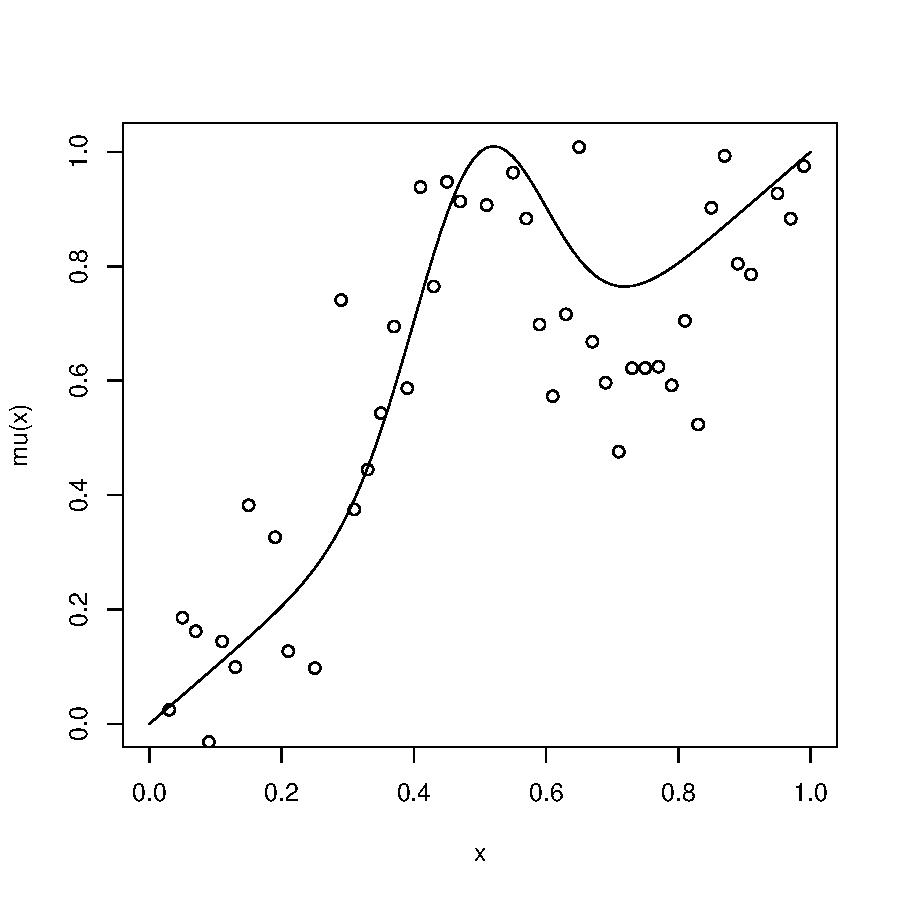
\includegraphics{EDA_Midterm_Exam-load_data}


\begin{enumerate}

\item For any regression estimator $\hat{\mu}(t)$ verify the identity

\begin{align*} R(\hat{\mu}) &= \frac{1}{n}  \sum_{i=1}^{n} \E [ \hat{\mu}(t_i) - \mu(t_i) ]^{2} \notag\\ 
&= \frac{1}{n}  \sum_{i=1}^{n} [ \E \hat{\mu}(t_i) - \mu(t_i) ]^{2} + \frac{1}{n} \sum^{n}_{i=1} \var(\hat{mu}(t_i))
\end{align*}


\item Using the function ksmooth() experiment with fitting various local kernel smoother estimators to this data by using both the box car kernel as well as the normal kernel by using kernel = "box" and kernel ="normal".  Note that when you type in $\text{fit}=\text{ksmooth}(x,y,\text{kernel}=\text{``normal'',bandwidth}=\text{lambda})$, fit\$y will return the fitted values $\hat{\by} = (\hat{\mu}_{\lambda}(t_1),\ldots,\hat{\mu}_{\lambda}(t_n))$.  Plot a scatter plot of the data, with the true value of $\mu(t)$ and overlay some plots of $\hat{\mu}_{\lambda}(t)$ for some visually promising values of kernel bandwidth's  $\lambda$.

\item  Write a program which will compute the cross-validation score as a function of smoothing parameter, where the cross validation score is given by
$$ CV(\lambda) = \frac{1}{lambda} \sum_{i=1}^{n} (y_i - \hat{\mu}_{\lambda (i)}(t_i))^{2} $$
where $\hat{\mu}_{\lambda (i)}(t_i)$ is the prediction of the model at the point $t=t_i$ which is trained on a dataset not containing the datapoint $(t_i,y_i)$ in the data set.  

\item Using your function, try several values of $\lambda$ and compute the associated value of $cv(\lambda)$. Once you have many pairs of $(\lambda, cv(\lambda))$ construct a plot using the smoothing parameter as the $x$-axis and $cv(\lambda)$ as the $y$-axis.  Your plot should be U-shaped, and based upon your plot select the smoothing parameter which minimizes $cv(\lambda)$.

\vskip.3cm\noindent
Now let's try something similar but for smoothing splines rather than kernel smoothers. In R you can use the function smooth.spline() under the stats package in R to fit a smoothing spline to data much like the following R code.  Under this model the fitted predcition has the form
$$  \hat{\by} = \BX \hat{\beta}  $$
where $\BX$ is the model matrix for the cubic B-spline basis.  The model matrix has the form where each column represents a different B-spline basis function $B_{j}(t)$ so the $(i,j)^{th}$ element of the $\BX$ matrix is given by $B_{j}(t_i)$. As the help function ?smooth.spline suggests, the coefficients $\hat{\beta}$ of the smoothing splines are computed by minimizing the penalized loss function
$$  L(\lambda) = (\by - \BX \beta)^{T} ( \by - \BX \beta) + \lambda   \beta^{T} \Omega \beta $$
where $\Omega$ is the smoothness penalzer matrix whose $(i,j)^{th}$ element approximates
$$  \Omega_{i,j} = \int_{0}^{1} B^{''}_{i}(t) B^{''}_{j}(t) dt .$$
The solution to this penalyzed loss minimization give
$$ \hat{\beta} = ( \BX^{T} \BX + \lambda \Omega )^{-1} \BX^{T} \by  $$
for the predicted B-spline regression coefficients and 
$$ \hat{\by} = \BS_{\lambda} \by =  \BX ( \BX^{T} \BX + \lambda \Omega )^{-1} \BX^{T} \by  $$
for the predicted value of $\by$.  The following R code can be used to generate approximate
values for all of these quantities (you should spend some time understanding what each of these R code
proceedures produce)

\begin{Schunk}
\begin{Sinput}
> sfit = smooth.spline(x,y,cv=TRUE)
> knots  = sfit$fit$knot
> # knots has several phantom knots 
> # at the boundary values of 0 and 1
> uniqueknots = unique(knots)
> library("fda")
> # to creat the X matrix you can use
> X = bsplineS(x,breaks=uniqueknots)
> # Or you can use
> X=splineDesign(knots,x)
> # regression coefficients are
> beta = sfit$fit$coef
> # you can get the approximate smoothness penalty matrix
> # by using
> B=create.bspline.basis(breaks=uniqueknots)
> Omega=bsplinepen(B)
> # Smoothing parameter is
> lambda = sfit$lambda
> # We can compute the Hat matrix by 
> #first inverting the matrix
> T=(t(X)%*%X+lambda*Omega)
> # Since T is a banded matrix this can be accomplished
> # efficiently using
> C= chol(T)
> Tinv = chol2inv(C)
> # Hat matrix is
> S = X %*% Tinv %*% t(X)
> # compare the sum of the diagonal of S with
> df = sfit$df
> df1 = sum(diag(S))
> # Regression coefficients are 
> betahat = Tinv %*% t(X) %*% y
>  # compare this to beta and you'll see they are close
> # the difference that are present maybe due to 
> # slight differences in Omega
\end{Sinput}
\end{Schunk}

\item  For several differnt values of the smoothing parameter, compare the quality of fit
    to the data by overlaying a plot of the smoothed prediction of the smoothing spline against the true 
    value of the mean $\mu(t)$ and the data.  What happens if $\lambda$ is small and big?
    
\item  For several values of $\lambda$ around the optimal value of lambda selected by the computer plot the $CV(\lambda)$ vs $\lambda$ and $GCV(\lambda)$ versus $\lambda$. Does it look like the optimal value of lambda selected by the computer minimimizes the each respective criterion? Is the GCV selected $\lambda$ the same as the CV selected lambda value?






\end{enumerate}


\end{enumerate}


\end{document}
